\documentclass{article}

\usepackage{graphicx}
\usepackage[margin=1in]{geometry}
\usepackage{booktabs}
\usepackage{float}
\usepackage{amsmath}

\begin{document}

\title{Rotation and Composition Findings}
\author{}
\date{12 February 2026}
\maketitle

\section*{Questions}
\begin{itemize}
    \item Is the composed kernel rotation invariant?
    \item Why is composite accuracy lower than the regular all-kernel model, and how can we reduce the gap?
\end{itemize}

\section*{Rotation-Invariance}
Composition is a weighted sum:
\[
K_{\text{comp}} = \sum_i w_i K_i
\]
This is not automatically rotation invariant. It becomes invariant only if the selected kernels and weights are rotationally balanced, or if the kernels are radially symmetric. Several kernel families used here are orientation-sensitive (e.g., anisotropic Gaussian, Gabor, HOG, LBP, GLCM), so the composite is expected to change under rotation.

Empirical checks on the saved composite kernel show large differences after 90$^\circ$/180$^\circ$/270$^\circ$ rotations. \textbf{Conclusion: the current composite kernel is not rotation invariant.}

\section*{Non-Invariant But Still Robust}
Even though the kernel itself is not rotation invariant, accuracy changes under 90$^\circ$ rotation were small:
\begin{itemize}
    \item Regular model: $\Delta$AUC $= +0.0017$, $\Delta$ACC $= +0.0123$
    \item Composite model: $\Delta$AUC $= +0.0086$, $\Delta$ACC $= +0.0241$
\end{itemize}

\textbf{Why accuracy stays stable:}
\begin{itemize}
    \item The response function \texttt{abs\_max} is insensitive to sign and location of the strongest response, so many rotations yield similar feature magnitudes.
    \item Logistic regression relies on pooled response magnitudes rather than explicit orientation alignment.
    \item Many kernels capture texture/contrast statistics that are preserved under right-angle rotations.
\end{itemize}

\section*{Why Composite is Lower}
\textbf{Best current results (12 February 2026):}
\begin{center}
\begin{tabular}{lcc}
\toprule
Model & Test AUC & Test ACC \\
\midrule
Regular (separate kernels) & 0.9376 & 0.8888 \\
Composite (8 kernels) & 0.9026 & 0.8299 \\
\bottomrule
\end{tabular}
\end{center}
\vspace{0.5em}
Training-stage AUC/ACC: regular 0.9243/0.8615 vs composite 0.9233/0.8541.

\begin{figure}[H]
    \centering
    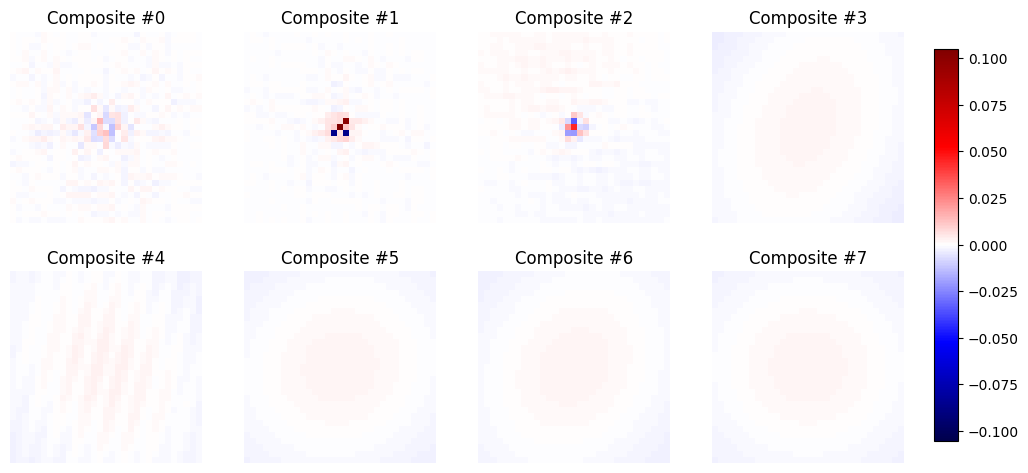
\includegraphics[width=0.9\linewidth]{../results/exp_022/composite_kernels_grid.png}
    \caption{Composite kernel grid (8 composites).}
\end{figure}

Main factors lowering composite accuracy:
\begin{itemize}
    \item \textbf{Feature collapse:} the regular model uses many kernel-response features; the composite reduces this to a small set, which compresses discriminative information.
    \item \textbf{Nonlinearity mismatch:} with \texttt{abs\_max} aggregation, composing kernels before response is not equivalent to combining per-kernel responses after \texttt{abs\_max}.
    \item \textbf{Heuristic weights:} composition weights are uniform or score-based, not optimized end-to-end for classification.
\end{itemize}

\section*{How to Reduce the Gap}
\begin{itemize}
    \item Use a \textbf{small bank of composites} (e.g., 8--32) instead of a single composite.
    \item Learn composition weights end-to-end with the classifier objective rather than using fixed heuristics.
    \item Make the response more linear (e.g., mean or sum pooling) so ``compose then respond'' is closer to ``respond then combine.''
    \item If strict rotation invariance is required, tie weights across rotated kernel orbits; note this may reduce accuracy if orientation cues are informative.
\end{itemize}

\section*{Qualitative Evidence (Heatmap Pairs)}
The following examples show side-by-side kernel and composite response visualizations for selected images. They illustrate how composition preserves some structure but can smooth or redistribute fine-grained responses.

\begin{figure}[H]
    \centering
    \begin{minipage}{0.48\linewidth}
        \centering
        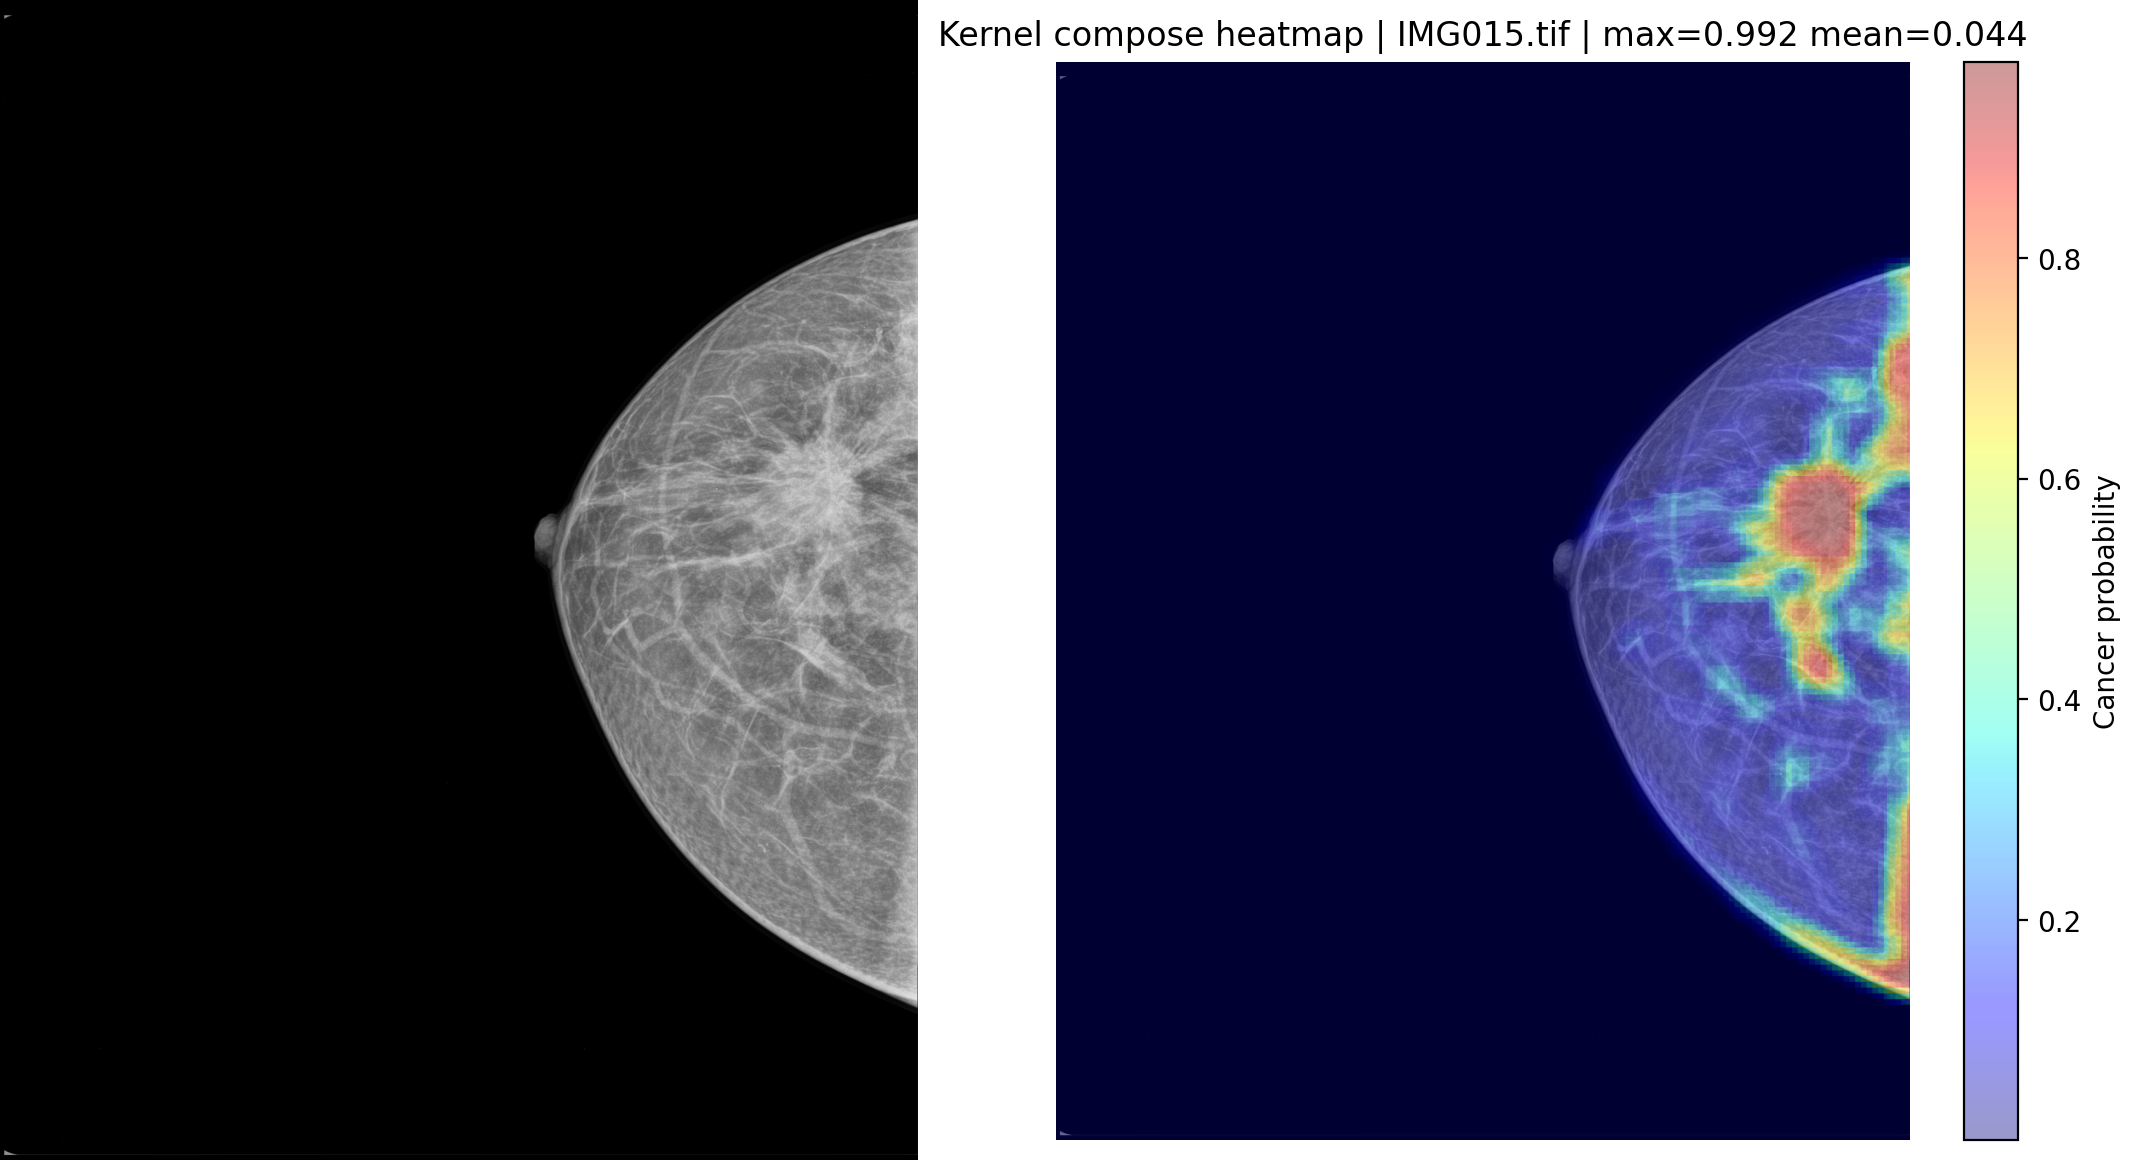
\includegraphics[width=\linewidth]{../results/exp_022/heatmaps_pairs/IMG015_kernel_compose_pair.png}
    \end{minipage}
    \hfill
    \begin{minipage}{0.48\linewidth}
        \centering
        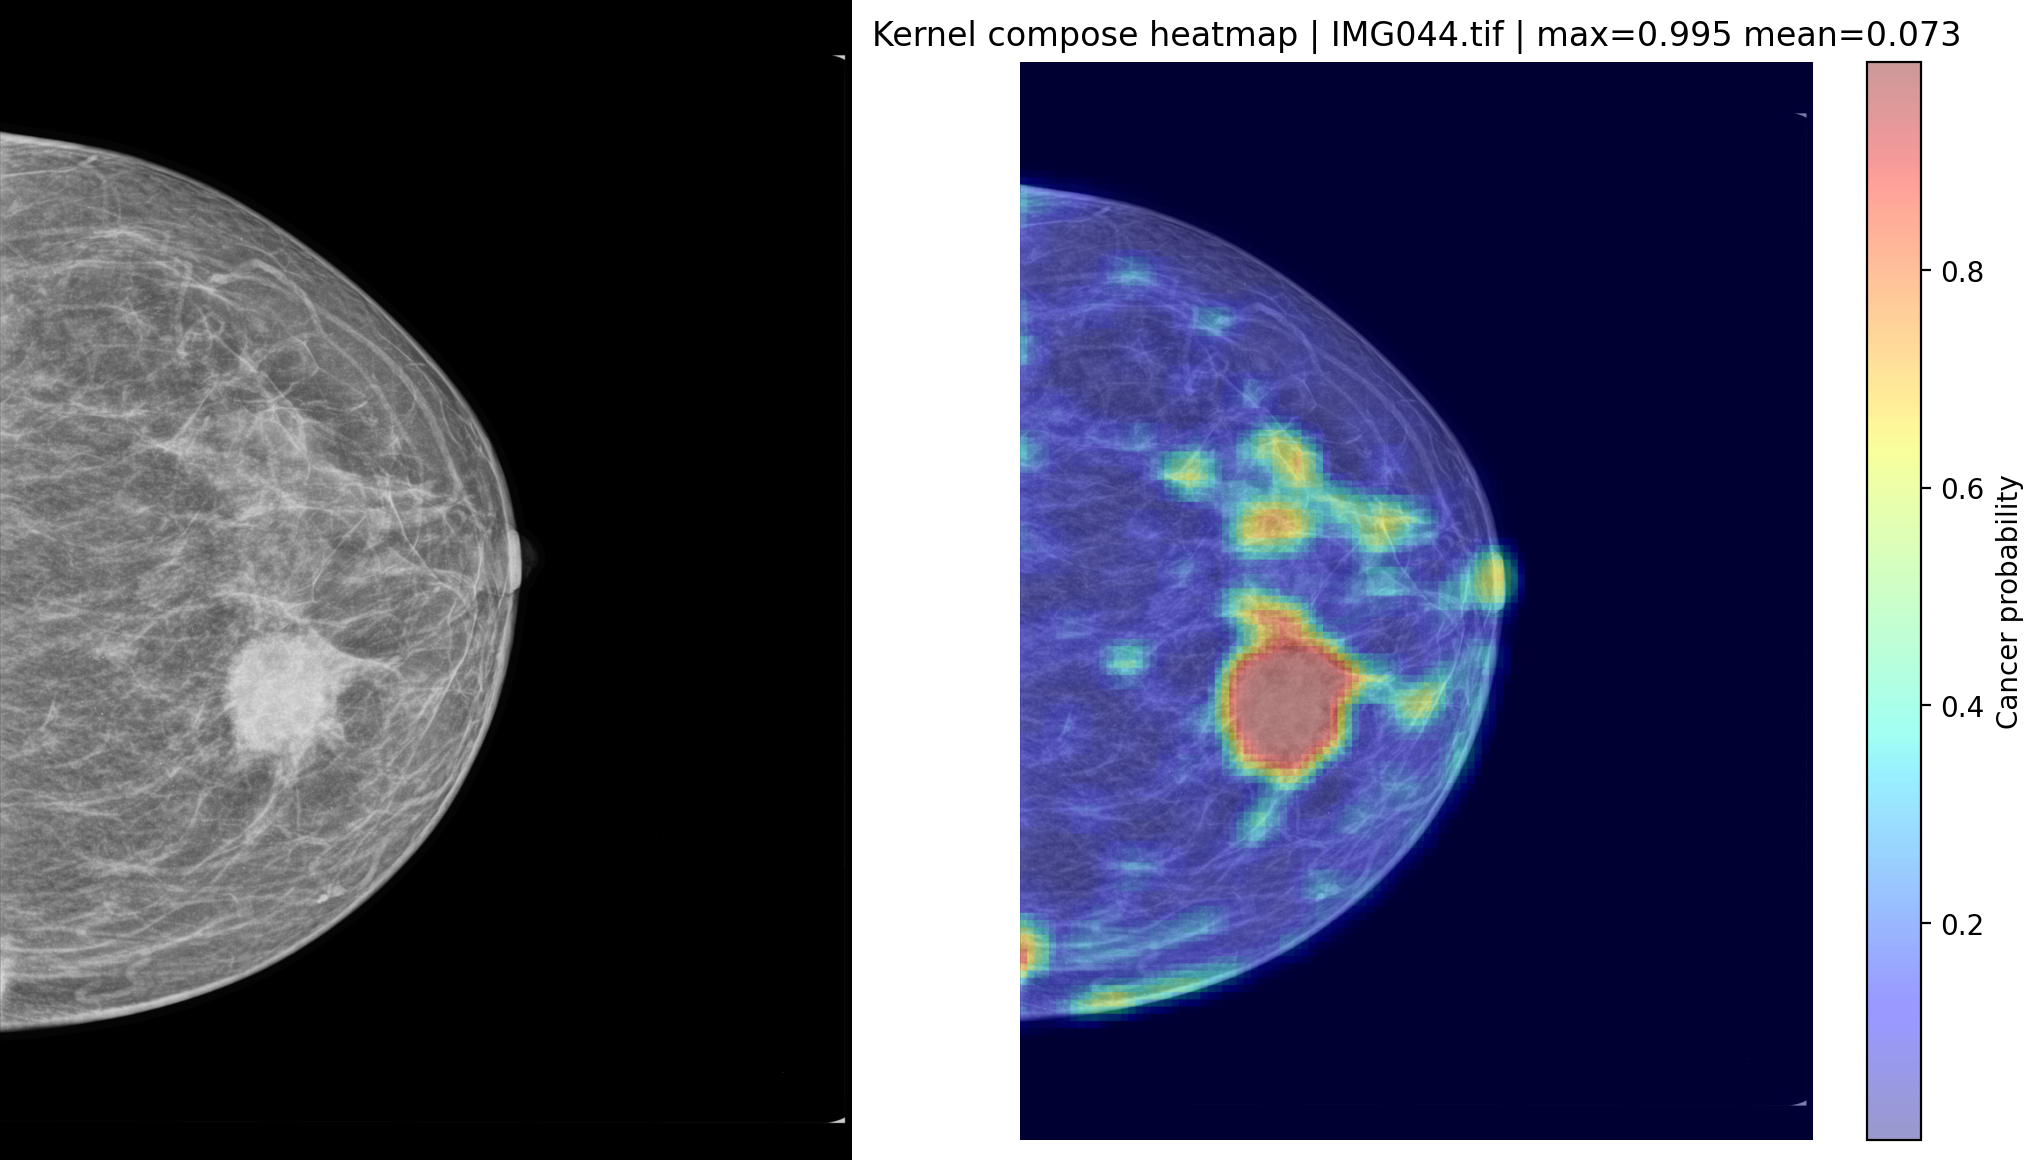
\includegraphics[width=\linewidth]{../results/exp_022/heatmaps_pairs/IMG044_kernel_compose_pair.png}
    \end{minipage}

    \vspace{0.5em}

    \begin{minipage}{0.48\linewidth}
        \centering
        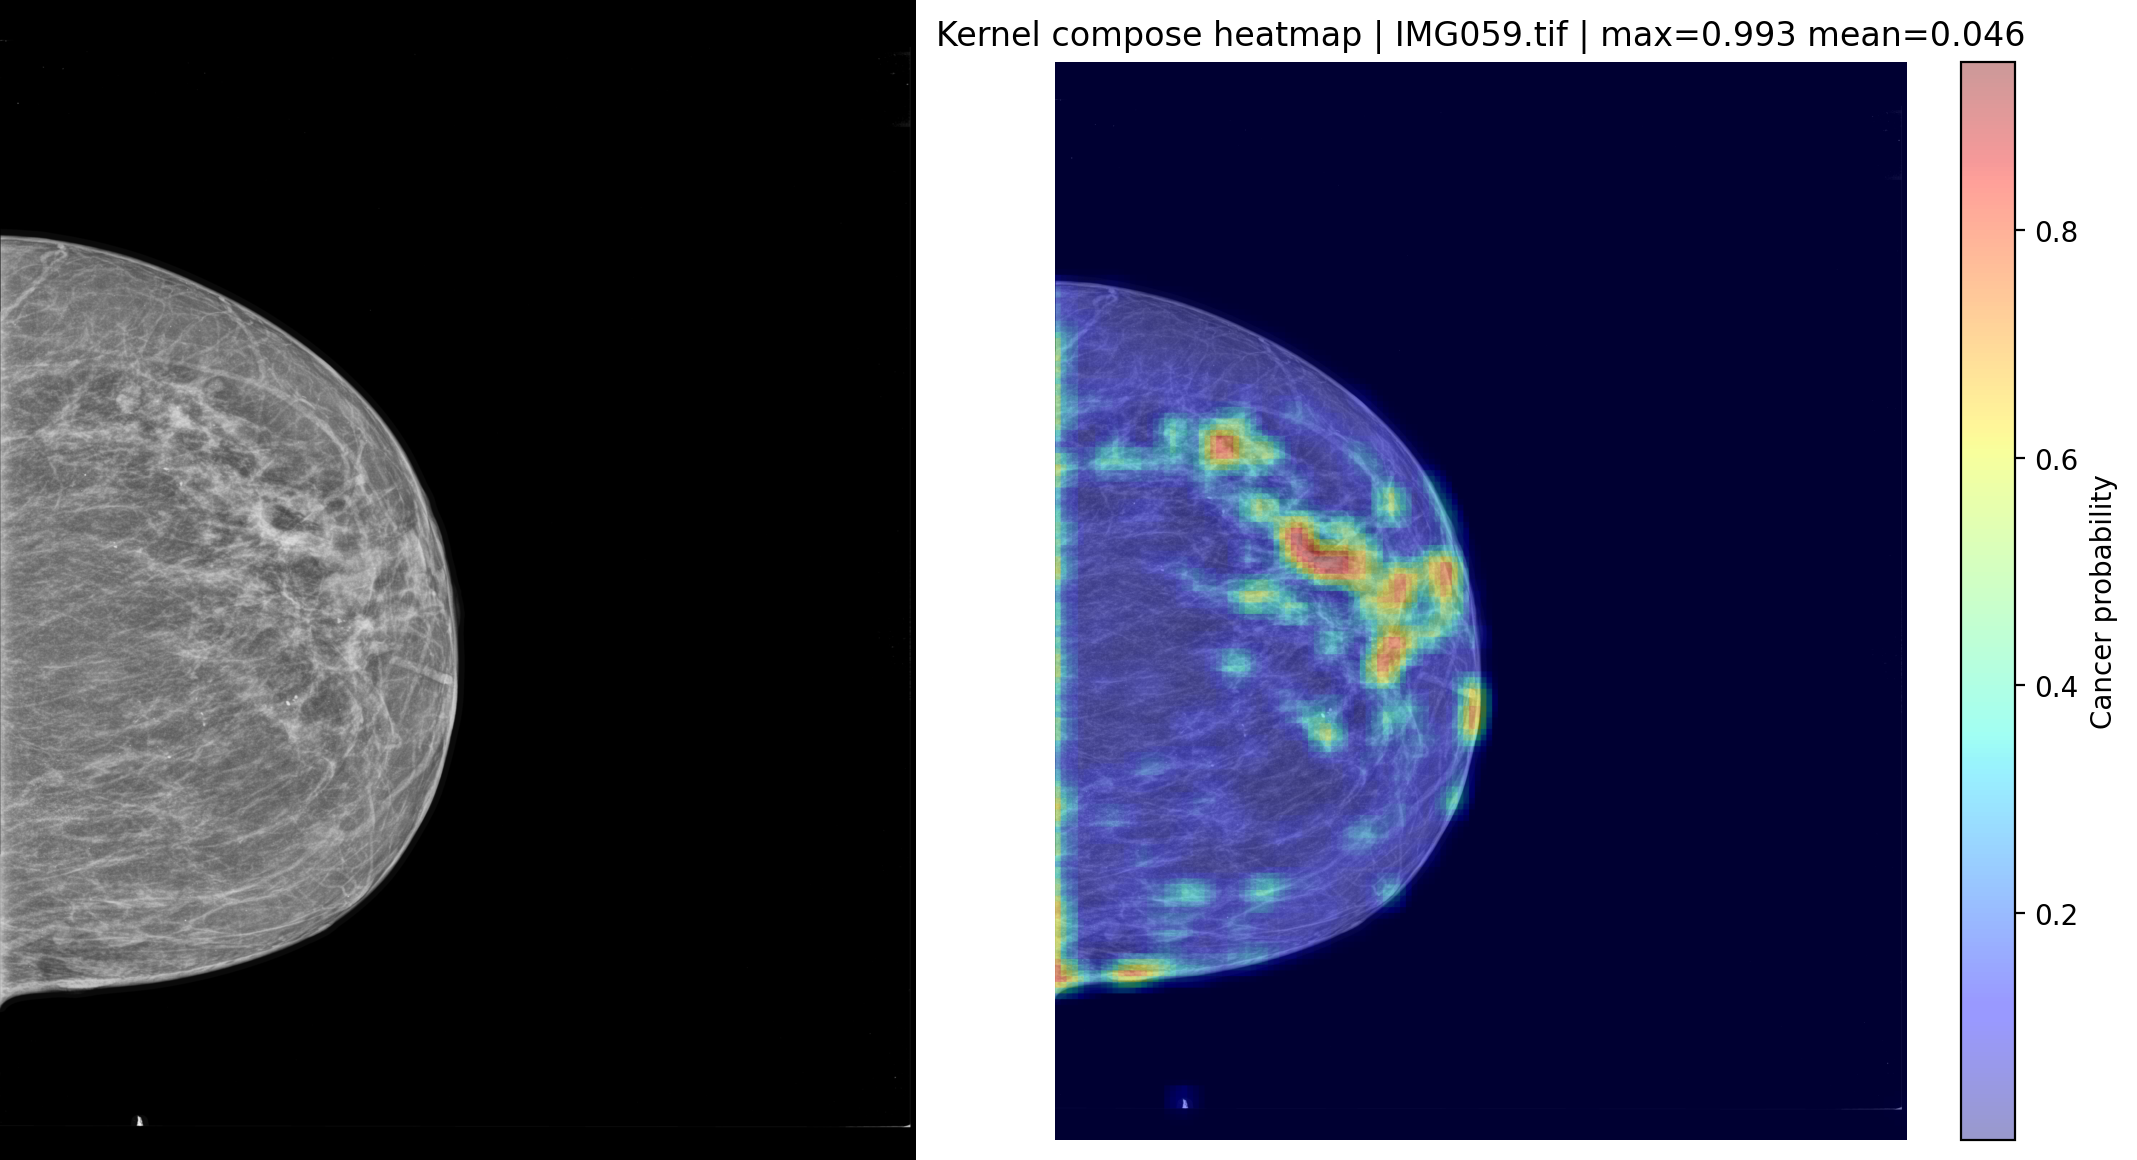
\includegraphics[width=\linewidth]{../results/exp_022/heatmaps_pairs/IMG059_kernel_compose_pair.png}
    \end{minipage}
    \hfill
    \begin{minipage}{0.48\linewidth}
        \centering
        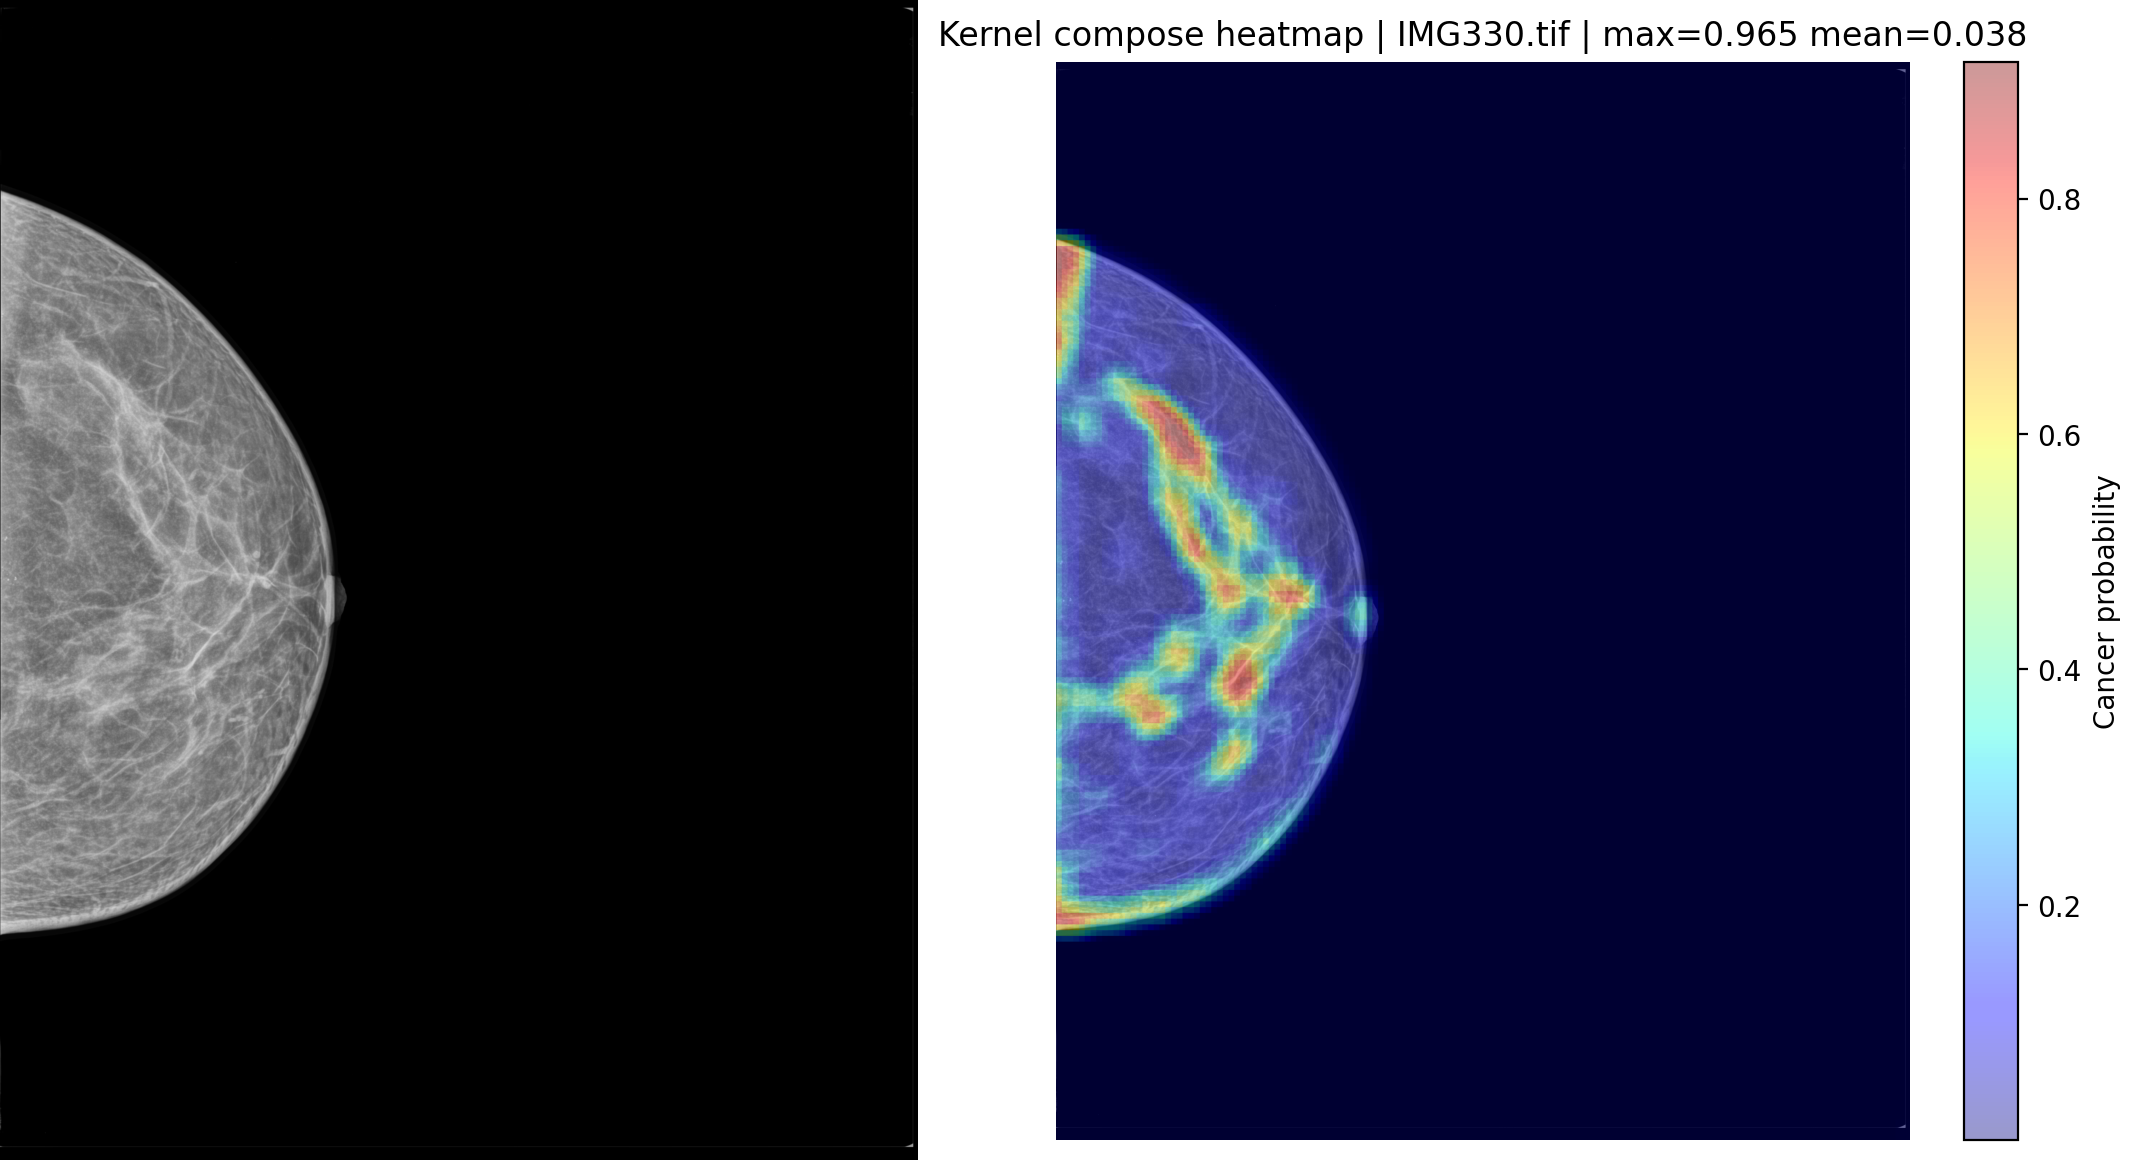
\includegraphics[width=\linewidth]{../results/exp_022/heatmaps_pairs/IMG330_kernel_compose_pair.png}
    \end{minipage}
    \caption{Kernel vs composite heatmap pairs for representative images.}
\end{figure}

% \section*{Why It Looks ``Zoomed''}
% The apparent magnification in composite-kernel visualizations is not a true geometric zoom (kernel size is unchanged). It is largely a spectral/superposition effect:
% \begin{itemize}
%     \item Summing many diverse kernels shifts energy toward lower frequencies and cancels fine detail.
%     \item L1/L2 normalization and per-plot color scaling can amplify the visual impression of larger, smoother patterns.
%     \item Mixed orientations and frequencies can create interference patterns (stripes/checkers).
% \end{itemize}

\section*{Current Pipeline and Next Step}
\begin{itemize}
    \item Current: kernel generation is random across parameter ranges.
    \item Change: smarter sampling using QMC or Latin Hypercube.
    \item Current: normalization is applied to composed kernels; non-composed kernels are used without an extra normalization stage. Prior runs without extra normalization performed better.
    \item Change: test per-family normalization (different normalization per kernel type).
\end{itemize}

\section*{Conclusion}
\begin{itemize}
    \item The current composite kernel is not rotation invariant, yet accuracy remains stable under 90$^\circ$ rotations.
    \item Composite accuracy is lower mainly due to feature collapse and nonlinearity mismatch.
    \item Closing the gap is more realistic with multiple learned composites than with a single kernel.
    \item Larger composition pools can look ``zoomed'' due to cancellation and normalization effects.
\end{itemize}

\end{document}
